\chapter{Introduction}
\label{cha:introduction}

%\chapterquote{I'm awesome!}{Barney Stinson, WIRED magazine, 19.1.2009}
Nowadays the every day's life of an individual is strongly influenced and/or supported by embedded devices, with or without them noticing it. These devices are more and more common, can have various shapes, and fulfill a very large number of functions. Among the most famous uses of embedded devices,  one can count automotive systems, mobile phone devices, or tracking systems.

On top of that, a new trend has emerged, where devices are interconnected and often autonomous, capable of communicating between each other. This is the case in the Internet of Things (IoT), where devices possess a web interface and communicate through the Internet. With such a network, features like knowledge-sharing, remotely triggered action or even decision-making are enabled. In theory, the capabilities of the IoT knows few boundaries and could be used in numerous future applications. 

In \citetitle{Atzori2010} \cite{Atzori2010}, Luigi Atzori et Al. pointed out that although the IoT has still to face some issues, like security and privacy, it could indeed benefit to many domains, like transportation and logistics, health-care, smart environments or the personal and social domain. For instance, such networks of devices begin already to be used for tracking purposes, assisted driving, mobile ticketing, augmented maps or smart homes but it could also be used in futuristic application, like robot taxi or enhanced game rooms. 

In addition, mobile devices (like mobile phones) have steadily growing capabilities, enhancing the features of IoT. These phones can for instance use a network of devices, or act as one node of the network. In the augmented maps example, hovering a tag with the mobile phone would trigger a web service call that would provide the device owner information about any point of interest, as hotels, restaurants, monuments or events. Such an integration of mobile devices into distributed systems leads to the fact that the computation could happen anywhere (or everywhere) and in any format. In other words, it leads to Ubiquitous Computing, often described as pervasive computing and explained by Mark Weiser as "Specialized elements of hardware and software, connected by wires, radio waves and infrared, will be so ubiquitous that no one will notice their presence" \cite{Computer_21Century}.

The Ubiquitous Computing is not something new, but it is getting more and more traction as the technologies, hardware or software (like middleware libraries) evolve. Jan Krikke assesses that "Interest has shifted from desktop computers to mobile computers such as cell phones, wearable computers, and advanced PDA-like devices such as Ubiquitous Communicator terminals"\cite{Krikke2005}. It can be therefore assumed that embedded and interconnected devices will be more and more present in the future.

In their paper, luigi Atzori et Al. also identify open issues that remain yet to be tackled for a better IoT. The IoT shows a need for standardization, as researches are conducted in many different places; it also has to respond to networking and addressing issues, since the IoT will inexorably lead to a number of network nodes that cannot be handled by the existing architectures and protocols (IPv4 for example is too limited in terms of addresses range). The last issue is the security and privacy one. The security theme encompasses protection against physical attack of the devices,  protection against eavesdropping, authentication of the different components, and data integrity. Privacy is the fact that personal information should be kept secret, or given to only authorized entities. 

Authorization and authentication are therefore one of the main issues in distributed system applications. 

The way both were handled in distributed systems evolved a lot in the last decades. In the past, a user had one password per service for which it had to be authenticated. As the number of such systems was restrained, this could work fairly good. But this system is not really scalable. In a big distributed system, having one password per user and per service require much effort from the user and a lot of capacity for the service providers. 

Recently, the term Single-Sign-On (SSO) appeared, in which a user authenticates just once for a set of different services. Google and Facebook, for example, implemented such a system, i.e., when a user wants to access a service X, instead of creating an account and signing in for X, it can simply connect to its Google Account and then access X. Of course the underlying process may be more complicated, but from the user's point of view, it isn't. Besides, the service providers like X don't have to maintain credentials for every user. For them, the system is also made easier.

But such an authorization and authentication system may be complicated to set up in a proper manner. Trust, efficiency, completeness are example of issues that must be taken into consideration. This thesis will mainly discuss the design of such an authentication and authorization framework within a specific network. 

\section{Context of this thesis}

This thesis is actually based on a possible future e-health application, where devices are shared among users: in telemedicine applications sensors are used to monitor vital signs of patients. The sensors belong to a specific entity (they could most likely be properties of the patient itself, or of a provider in case of research study for example), and the data collected by the sensors can be retrieved from the Internet in case another entity, like an hospital, wants to have access to the vital signs. 

Nevertheless, in case of real-time data like vital signs, it is better to have a direct access to the sensors and be able to read the data from them. This way, problems like delay or data corruption can be avoided, or at least lowered. The sensors should then be shared among customers, and one could also imagine a billing system like Pay-As-You-Go. Such a system is further on called \emph{devices cloud}. A global system has already been designed, described in details in the following thesis: \citetitle{reference_thesis} \cite{reference_thesis}.

One of the security issue that this \emph{devices cloud} and the IoT share is the fact that a device is physically present, and can therefore be directly attacked and destroyed. A device has namely a physical representation and a virtual one, used for communicating with the other devices. This is one of the key difference of such a system in regards to more standard approaches of Internet based network, like cloud-based system, where the only thing a user can have access to is the virtual representation of a network node. For instance, With Dropbox or Amazon EC2, two of the most famous cloud-based system, the only thing that one has access to is indeed a web interface.

The device existing as a physical object leads also to the fact that it actually belongs to someone or to an entity, and should by laws be handled (in the sense of using, renting or selling) by the same entity. This aspect should be taken into consideration when sharing the devices, i.e. granting a customer with the right to use the sensors.

In the proposed solution, many actors interact between each other. For the purposes of this thesis, the following roles are particularly important:

\begin{description}
	\item[Device Owner]: the entity that owns the particular device
	\item[Device Consumer]: the entity that is requesting access for the purpose of reading data from the device or controlling it
	\item[Device Operator]: the entity that operates or manages the device provisioning in charge of the Device Owner. The Device Operator can also hold the Device Owner's role
\end{description}

The Operators, providing access to the devices (as service providers), also act as peers and have contracts between each other to provide access for their customers to a device operated by another Operator.

Of course, the \emph{device cloud} must implement an authentication and an authorization layer to grant the right entity with the corresponding rights. As aforementioned, the access to a device is an example of a right that must be granted. This thesis will have for goal to design a robust authentication system responding to the devices cloud needs and fitting the roles and entities defined in such a cloud. 


\section{The problem}
The complexity of the authorization and authentication system is at least threefold: it lies in the variety of actors and entities, in the variety of existing solutions and protocols, and in the restrictions inherent to the devices.

\subsection{Various actors} 
For better understanding of which entity must be handled, a simplified structure of the \emph{devices cloud} is depicted in Fig \ref*{fig:concept__architecture}. This architecture, which will be thoroughly explained in chapter \ref{cha:relatedwork}, includes the following entities:
\begin{itemize}
	\item Consumer
	\item Aggregator
	\item Consumer Operator
	\item Domain Operator
	\item Root Domain Operator
	\item Vendor
\end{itemize}

\begin{figure}[!ht]
	\centering
	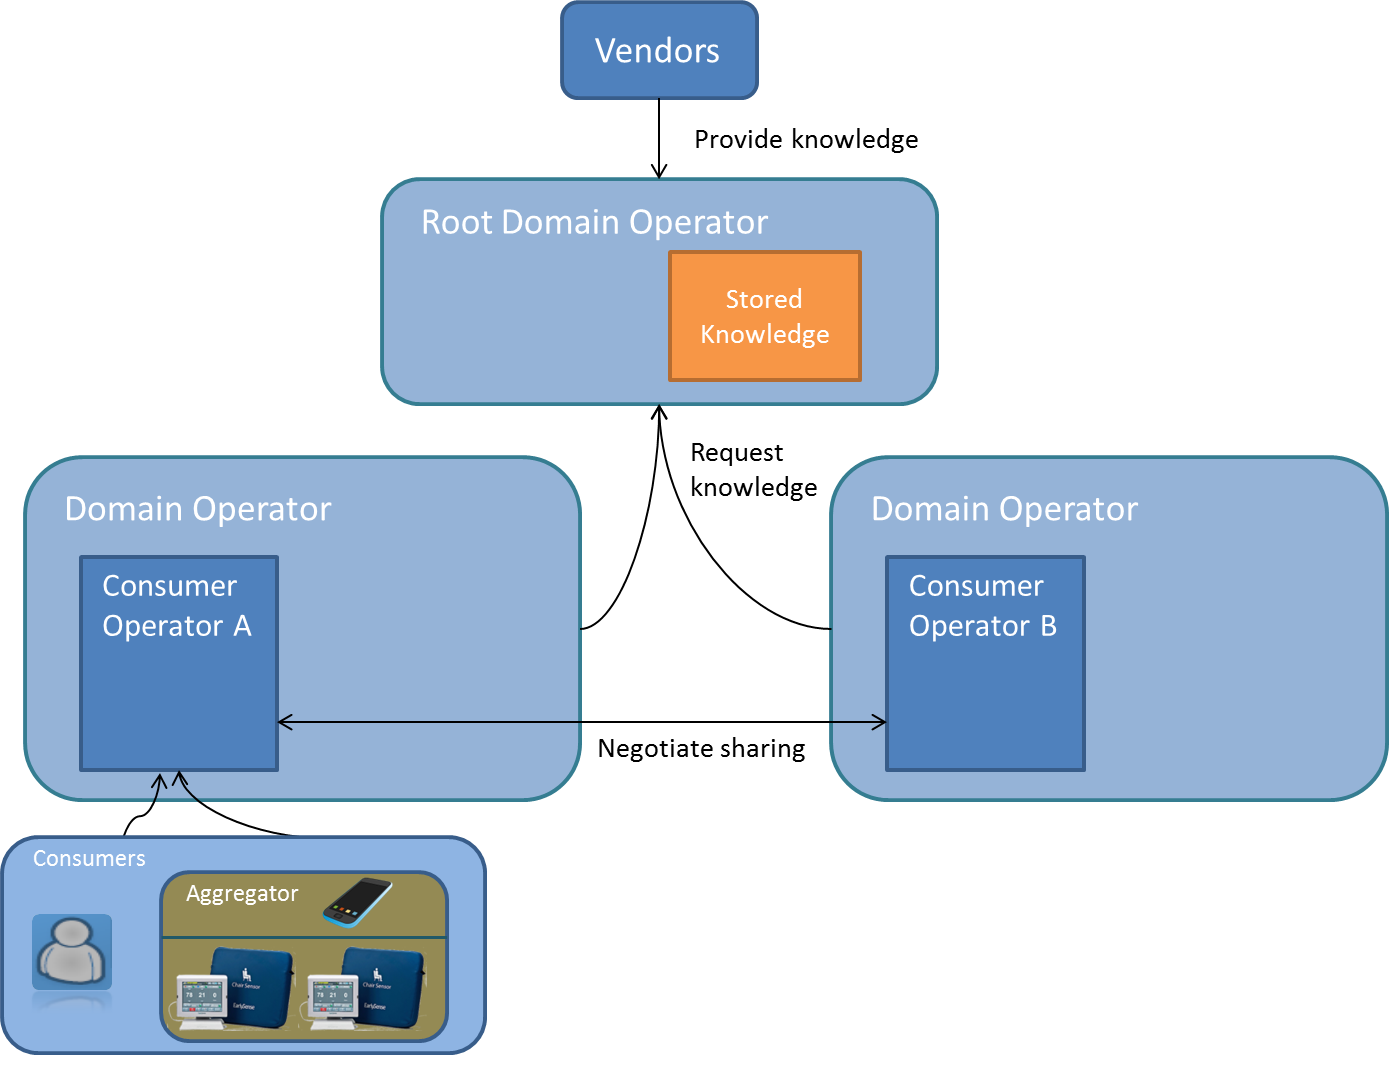
\includegraphics[width=0.8\textwidth]{images/design.png}\\
	\caption{Global architecture}
	\label{fig:concept__architecture}
\end{figure}

In this architecture, the Domain Operators take the role of Device Operator and act as service providers. The devices they operate are grouped within aggregators, a virtual layer (software entity) that integrates devices and which is generally situated where the devices are. Typically, a consumer's mobile phone plays the role of the Aggregator and allows the consumer to handle every device. It contains among other the required middleware for loading the drivers and software that a device needs, and for establishing a reliable communication channel between the devices and the other actors. Since aggregators communicate with other entities, it has to be authenticated.

Besides, the process of provisioning a device involves several steps and management services like accounting or decision making. In order to hide this complexity from the end users (i.e. Consumers), an Operator, called Consumer Operator, has been introduced. A Domain Operator can have several Consumer Operators, each handling different customers and devices. When a customer wants access to a device, it requests its Consumer Operator first. The customer, requiring access to a protected resource, needs to be authenticated. 

It can happen that the Consumer Operator doesn't operate the specific device. In this case, it must request which other Consumer Operator owns the device. Once it will have retrieved this information, if the two Consumer Operators are bound by a contract, the device's access can be provided. Of course, the requesting Customer operator must be authenticated within the Domain of the other one.

In the previous scenario, the Consumer Operator needs to know which other Consumer Operator handles a specific device. For this request to succeed, global knowledge has to be stored. Which device is operated by which operator for example. In the same way, it is assumed that the Operators are provided with all the knowledge which is required for operating a device. But when integrating a new unknown device, this knowledge must be first retrieved. \\Therefore, in the already defined system, two other entities have been introduced: the so-called Root Domain Operator is placed on top of the Domain Operators and stores global knowledge about devices and existing Operators; the Vendor Entity represent vendors (of devices), which are part of the global process and furnish knowledge about the different devices. Since the Vendors communicate with the Root Domain Operator about protected and required knowledge, it must also be authenticated within the Root Domain Operator. 

When the Consumer Operator requests which other Consumer Operator operates a specific device, the requesting Consumer Operator acts for the Root Domain Operator as a client requesting access to a protected resource, and must then be authenticated by the Root Domain Operator.

In the end, four entities must be authenticated: the Consumers, the Aggregators and the Consumer Operators must be authenticated within Domain Operators, the Vendors and the Consumer Operators within the Root Domain Operator.

The different processes among the \emph{devices cloud} involve also roles and authorization. An example for that is access revocation, which could be needed in the following case: an emergency occurs requiring customer A to have control over device D, but customer B is using the device D at that time. The access must then be revoked before the device is re-attributed to customer A. In this case, only the Device Owner or Device Operator can take such a decision. Roles and authorization must therefore be handled.

\subsection{Different Technologies}
Concerning the technology that will be used, several choices are possible. One could rely on a Password-authenticated key agreement \cite{Hao2011}\cite{Pointcheval2012}\cite{Juang2008}, symmetric or asymmetric encryption\cite{Woo1997}\cite{Denning1982}, on the Diameter protocol, the kerberos protocol\cite{Sundareswaran}, the Otway–Rees protocol, openID\cite{Ghazizadeh} and openID connect, SPX\cite{Tardo1991} or some others. A. Liebl tried in 1994 to list the possible authentication protocols, his list is given in appendix 1.

It has been decided to use OpenID Connect as authentication framework (with Oauth as authorization frameworkt).

After the protocol has been chosen, it should be decided if the implementation must be done from scratch, or with help of libraries. The use of libraries facilitates the implementation, but it should be reminded that this work will eventually be integrated into an already existing bigger project. In that sense, homogeneity and transparency are also issues that one has to consider. 

In this thesis, MitreID, a Java library, has been elected.

{ \huge TODO: REVIEW THE SOLUTION }

%Regarding breaches and potential attack when it comes to distributed systems, it seems that a few possibilities stand out: a Kerberos based system, an OpenID system, or a system based on an OAuth protocol (like OpenID connect). More details will be given is chapter \ref{cha:conceptanddesign}.



%If the use of libraries is chosen, the a specific library should be elected. Talking about OpenID connect, which is quite recent, six libraries at least are available. Kerberos, a much older protocol, can be implemented from basically any existing security framework. 

\subsection{Devices Restriction}
When implementing an authentication and authorization layer in the \emph{devices cloud}, it should be taken into consideration that a part of the implementation will eventually run on the devices platforms. 

Within these platforms, resources are scarce and computation power low. Hence, heavy-weight libraries and protocols should be avoided.

\section{Aim and Objectives}
Every Domain Operator (Root or not) should be then able to authenticate other actors of the \emph{device cloud}.

For that, a User Directory should be designed. This User Directory is maintained locally by every Domain Operator for authenticating their own "users" (which can be one of the four entities described above). The User Directory used in the \emph{device cloud} should have the same implementation for every Domain Operator, and thus should implement the required level of abstraction to be used indifferently in any Operator.

For the system to be complete, a client side (requesting authentication) will be also implemented. This client will for example be used by the vendors or the consumers and will communicate with the User Directory of their Operator. As said above, this client should be deployed onto the devices platform and should be thus be kept as light as possible.

It should also be decided if this User Directory relies within each operator on a dedicated database (storing users, session information) or if it should be wrapped onto an existing IAM (Identity and Access Management) solution, or onto a LDAP for instance. In our case, the authorization and authentication framework is based on a dedicated database.
{ \huge TODO: REVIEW THE SOLUTION }

Since several Domain Operators exist at the same time, it is legitimate to specify where should which entity's record be kept. For example, a Consumer Operator is susceptible to communicate with any other Operator. Therefore, a Domain Operator can have in its User Directory an entry for any other Operator. On the contrary, a Consumer or an Aggregator is supposed to communicate only with its Operator. It is subsequently mandatory, that a Domain Operator stores information only about their own consumers and aggregators. In the same way, vendors information should be only stored in the Root Domain.

M. Mackay et Al. recently identified the major threats in a cloud-based system as\cite{Mackay2012}: 
\begin{enumerate}
	\item Hacking attacks
	\item DDoS attacks
	\item Insider attacks
	\item Equipment failures
	\item End-to-end issues
	\item Espionage
	\item Data loss or corruption
\end{enumerate}

To those threats the risks related to the physical presence of sensors like destruction or damaging(8) can be added .

As for the User Directory, the design should respond to the issues 1, 6 and 7. The DDoS attacks(2) are performed on the network, and thus cannot be prevented by the design of a single component. The same argument can be given for end-to-end issues(5). Equipment failures(4), as equipment destruction or damaging(8), are absolutely not related to the design and implementation of a User Directory. Hence, it is out of the scope of this thesis. 

Handling with insiders attacks is more about predicting and detecting than preventing, and is based on observation of patterns and users behavior that are not visible to the User Directory\cite{Schultz2002}. However, it can be ensured that an authorized participant cannot access protected information with which it could harm the system.

Hacking attacks, Espionage and Data loss or corruption can be handled through data encryption, signatures, or other security standards (handling SQL injection, XSS attacks, etc). Thus, it must be ensured that the User Directory provides a sufficient security level in regards to those issues, while being easily integrable into the global design. 

Finally, privacy should be also ensured.


\section{Outline}
After the introduction to this thesis and its related background, BLABLABBLA

Chapter 2 BLABLABBLA

Chapter 3 BLABLABBLA

CHapter 4 BLABLABBLA

Finally, BLABALABAKA



